% =============================================================================
% TG-1 Presentation — Undergraduate Thesis Proposal
% Hawkes process parameter estimation via neural networks on high-frequency
% cryptocurrency data.
% Theme: Mid-Century Modern (DeepBlue). Compile with: xelatex (3x).
% =============================================================================
\documentclass[aspectratio=169]{beamer}
\usepackage{beamerthememidcenturymodern}
\usepackage{graphicx}
\usepackage{booktabs}
\usepackage{amsmath,amssymb}
\usepackage{tikz}
\usetikzlibrary{arrows.meta,positioning,shapes.geometric,fit,backgrounds}

\mcmTheme{DeepBlue}
\mcmTitleUppercasefalse
\mcmSectionNumberMarkerOff

% --- title-page sizing (keeps title/date on screen) ---
\setbeamerfont{title}{size={\fontsize{19}{22}}, series=\bfseries}
\setbeamerfont{subtitle}{size=\normalsize, series=\mdseries}
\setbeamerfont{author}{size=\large}

% --- lightweight citation marker (no biblatex on this toolchain) ---
\newcommand{\cit}[1]{{\footnotesize\color{mcmPrimary}[#1]}}

% --- Metadata ---
\title{Hawkes Process Estimation on High-Frequency Cryptocurrency Data via Neural Networks}
\subtitle{From recurrent LSTMs to attention-based architectures}
\author[João Matheus]{\textbf{João} Matheus Del Vecchio}
\institute{Advisor: Prof.\ Dr.\ Mauri Aparecido de Oliveira\\ Instituto Tecnológico de Aeronáutica — Computer Engineering}
\date{June 2026}

\titlegraphic{
  \begin{minipage}{0.21\linewidth}
    \begin{center}
    
\includegraphics[width=3cm]{logos/ita_logo.png}
    \end{center}
  \end{minipage}
}

\AtBeginSection[]{%
  \begin{frame}[plain]
    \sectionpage
  \end{frame}
}

\begin{document}

% =====================================================================
\begin{frame}
  \titlepage
\end{frame}

% =====================================================================
\begin{frame}{Table of Contents}
  \tableofcontents
\end{frame}

% =====================================================================
\section{Context}
% =====================================================================
\begin{frame}{Context — why do prices move?}
  \begin{block}{Volatility \emph{is} activity \cit{Bouchaud et al., 2018}}
    Minimal microstructure model: the price moves by $\pm\vartheta$ (one tick) at a rate $\phi$ per unit time (the market \textbf{activity}), with up and down moves equally likely. The price volatility is then
    \[
      \boxed{\;\sigma^2 = \phi\,\vartheta^2\;}
      \qquad\text{(Bouchaud et al., 2018, Eq.\ 2.18).}
    \]
  \end{block}
  \begin{itemize}
    \item To first order, \textbf{volatility is the rate $\phi$ of price-change events}.
    \item Modelling volatility $\;\equiv\;$ modelling the \textbf{intensity $\phi$} of a point process.
  \end{itemize}
  \begin{alertblock}{Consequence}
    If $\phi$ varies randomly in time, then \textbf{volatility is stochastic} — with its own dynamics.
  \end{alertblock}
\end{frame}

\begin{frame}{Context — volatility is stochastic and clustered}
  \begin{block}{The empirical fact}
    Activity (hence volatility) is \textbf{intermittent}: it alternates calm and bursts, with \textbf{long memory} (\emph{volatility clustering}) \cit{Bouchaud et al., 2018}.
  \end{block}
  \begin{columns}[T]
    \begin{column}{0.55\textwidth}
      \begin{block}{Point-process formalism}
        \begin{itemize}
          \item $N(t)=\sum_i \mathbf{1}_{t_i\le t}$ counts events; intensity $\phi(t)=\mathbb{E}[\mathrm{d}N(t)]/\mathrm{d}t$.
          \item \textbf{Clustering ratio}: $\;r(\tau)=\dfrac{\mathbb{V}[N(t{+}\tau){-}N(t)]}{\mathbb{E}[N(t{+}\tau){-}N(t)]}$.
          \item Inter-event durations: cf.\ ACD models \cit{Pacurar, 2006}.
        \end{itemize}
      \end{block}
    \end{column}
    \begin{column}{0.45\textwidth}
      \begin{alertblock}{Poisson is not enough}
        A homogeneous Poisson process ($\phi$ constant) gives $r=1$ (no clustering). In markets, $r\gg 1$: the intensity $\phi=\phi(t)$ must be \textbf{stochastic}.
      \end{alertblock}
    \end{column}
  \end{columns}
\end{frame}

\begin{frame}{Context — the Hawkes process}
  \begin{columns}[T]
    \begin{column}{0.54\textwidth}
      \begin{block}{The intensity becomes its own model \cit{Hawkes, 1971; intro: Muni Toke, 2011}}
        \[
          \phi(t)=\underbrace{\phi_0(t)}_{\text{exogenous}}+\underbrace{\sum_{t_i<t}\Phi(t-t_i)}_{\text{endogenous (self-excitation)}}
        \]
        \begin{itemize}\footnotesize
          \item Each event raises $\phi$ by a kernel $\Phi\!\ge\!0$ that decays in time.
          \item As $\phi(t)$ depends on \textbf{its own history}, it is \emph{itself stochastic}.
          \item With $\sigma^2(t)=\vartheta^2\phi(t)$, \textbf{volatility becomes stochastic and clustered} \cit{Bouchaud et al., 2018}.
        \end{itemize}
      \end{block}
    \end{column}
    \begin{column}{0.46\textwidth}
      \begin{figure}
        \centering
        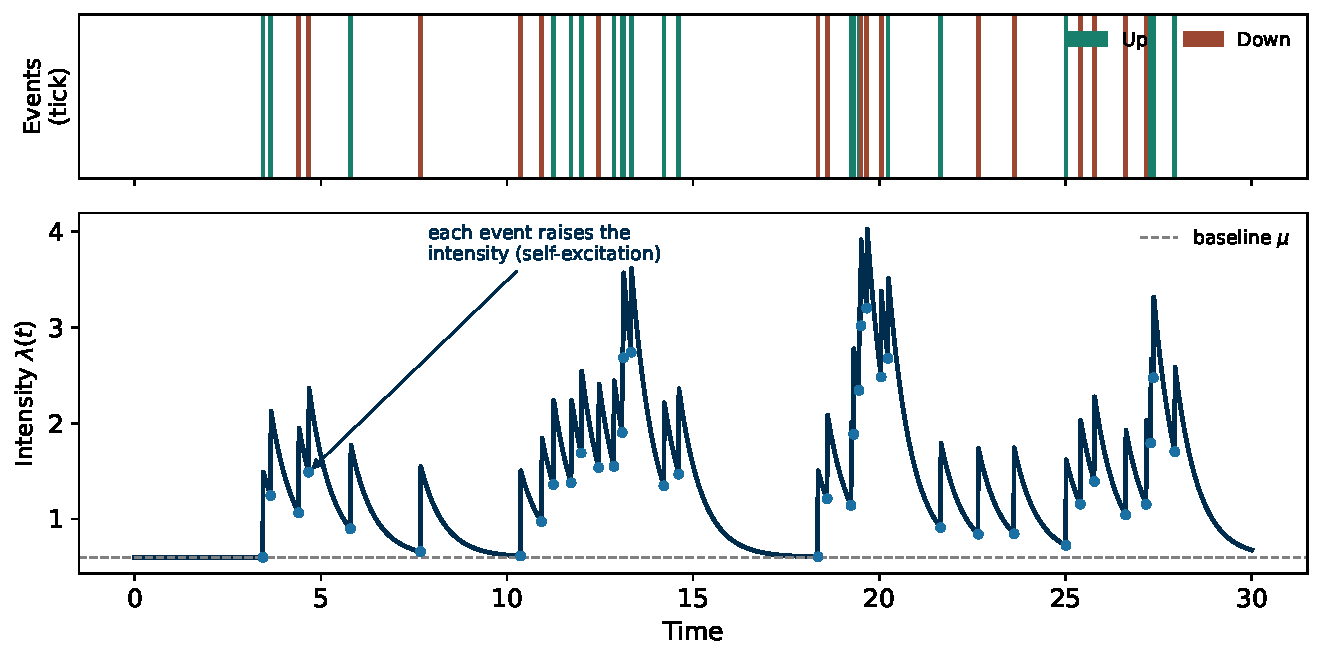
\includegraphics[width=\linewidth]{figs/fig_hawkes.pdf}
        \caption{Simulated Hawkes process: events (top) raise the intensity $\phi(t)$ (bottom), which decays until the next one.}
      \end{figure}
    \end{column}
  \end{columns}
\end{frame}

\begin{frame}{Context — endogeneity and reflexivity}
  \begin{columns}[T]
    \begin{column}{0.55\textwidth}
      \begin{block}{Branching ratio $g$}
        \[
          g=\int_0^\infty \Phi(u)\,\mathrm{d}u<1
          \;\Rightarrow\;
          \bar\phi=\frac{\phi_0}{1-g},\quad \bar S=\frac{1}{1-g}.
        \]
        \begin{itemize}\footnotesize
          \item Branching view: $g$ = expected number of ``child'' events each event triggers (mother $\to$ children).
          \item $g\to 1$: \textbf{near-critical} market, activity mostly \textbf{endogenous} (\emph{reflexivity}) \cit{Hardiman, Bercot \& Bouchaud, 2013}.
          \item The process memory grows as $1/(1-g)$.
        \end{itemize}
      \end{block}
    \end{column}
    \begin{column}{0.45\textwidth}
      \begin{block}{In our model}
        Exponential kernel $\Phi(t)=\alpha\,e^{-\beta t}$:
        \[ g=\alpha/\beta. \]
        Estimating $\{\mu,\alpha,\beta\}$ = measuring \textbf{baseline}, \textbf{feedback strength} and its \textbf{memory}.
      \end{block}
      \begin{alertblock}{Why it matters}
        Estimating Hawkes $\equiv$ measuring, interpretably, the market's \textbf{volatility} and its \textbf{degree of endogeneity}.
      \end{alertblock}
    \end{column}
  \end{columns}
\end{frame}

% =====================================================================
\section{Motivation}
% =====================================================================
\begin{frame}{Motivation}
  \begin{itemize}
    \item Hawkes estimation is traditionally done by \textbf{maximum likelihood (MLE)}: accurate and well-founded, but \textbf{iterative and costly}, sensitive to the initial guess and hard to use in real time.
    \item \textbf{Lee (2023)} \cit{Lee, 2023} proposes estimating the parameters with an \textbf{LSTM}: the network learns on simulated data and predicts the parameters directly — accuracy comparable to MLE, inference time $<1\%$ of MLE.
    \item Lee's study uses \textbf{US equities (2018--2019)}. The method is promising, but \textbf{little explored} in other markets and with \textbf{other network architectures}.
  \end{itemize}
  \begin{alertblock}{Gap}
    There is a lack of studies that (i) apply neural-network Hawkes estimation to \textbf{high-frequency cryptocurrency data} and (ii) investigate whether \textbf{attention-based architectures} improve estimation over the reference LSTM.
  \end{alertblock}
\end{frame}

\begin{frame}{Motivation — why cryptocurrencies?}
  \begin{columns}[T]
    \begin{column}{0.55\textwidth}
      \begin{block}{A fertile, challenging ground}
        \begin{itemize}
          \item A \textbf{24/7}, liquid market with \textbf{public tick data} (e.g.\ exchange order-book and trade dumps) — no cost for equity NBBO data.
          \item \textbf{Clustered jumps and heavy tails}: Hawkes outperforms Poisson for jumps in crypto \cit{Taddeo, Salvi \& Rivera-Castro, 2024}.
          \item An emerging market in Brazil, still little studied under this lens \cit{Primo, 2018}.
        \end{itemize}
      \end{block}
    \end{column}
    \begin{column}{0.45\textwidth}
      \begin{alertblock}{Opportunity}
        The more ``excited'' dynamics of crypto make it an ideal case to test whether \textbf{attention} models capture long-range dependencies better.
      \end{alertblock}
    \end{column}
  \end{columns}
\end{frame}

% =====================================================================
\section{Objectives and Hypothesis}
% =====================================================================
\begin{frame}{Hypothesis and Objective}
  \begin{alertblock}{Research hypothesis}
    A neural network can estimate the parameters of a marked Hawkes process from high-frequency cryptocurrency data with \textbf{accuracy comparable to maximum likelihood at orders-of-magnitude lower computational cost}; moreover, \textbf{attention-based architectures} can \textbf{match or surpass} the reference LSTM in estimation quality, especially under crypto's more clustered, heavy-tailed jump dynamics.
  \end{alertblock}
  \begin{block}{Main objective}
    Replicate and extend Lee (2023), applying it to crypto data and investigating alternative architectures (notably attention/Transformer) for parameter estimation and real-time volatility computation.
  \end{block}
\end{frame}

\begin{frame}{Specific objectives and scope}
  \begin{columns}[T]
    \begin{column}{0.55\textwidth}
      \begin{block}{Specific objectives}
        \begin{enumerate}\footnotesize
          \item Implement the 2D marked Hawkes model and the \textbf{MLE estimator} (baseline).
          \item Build the \textbf{simulator} (Ogata thinning) and the training-set generator.
          \item Reproduce Lee's (2023) \textbf{3-layer LSTM}.
          \item Adapt the pipeline to \textbf{real crypto data}.
          \item Design alternative architectures: \textbf{GRU, deep LSTM and attention/Transformer}.
          \item Compare \textbf{accuracy, time and robustness}.
          \item Apply to \textbf{intraday Hawkes volatility}.
        \end{enumerate}
      \end{block}
    \end{column}
    \begin{column}{0.45\textwidth}
      \begin{block}{Scope}
        \begin{itemize}\footnotesize
          \item \textbf{2D symmetric} Hawkes process with exponential decay and marks (jumps).
          \item \textbf{``High''} frequency (filtering at $\Delta t=0.1$\,s), not ultra-high.
          \item Focus on \textbf{parameter estimation} and \textbf{volatility}, not trading.
        \end{itemize}
      \end{block}
      \begin{alertblock}{Out of scope}
        Full limit-order-book modelling; price-direction forecasting; order execution.
      \end{alertblock}
    \end{column}
  \end{columns}
\end{frame}

% =====================================================================
\section{Theoretical Background}
% =====================================================================
\begin{frame}{Marked Hawkes price model}
  \begin{block}{Conditional intensity (2D, exponential decay)}
    \[
      \boldsymbol{\lambda}_t=\boldsymbol{\mu}+\int_{(-\infty,t]\times E}\boldsymbol{\alpha}\circ \boldsymbol{b}(t-u)\,\boldsymbol{M}(\mathrm{d}u\times\mathrm{d}z),
      \quad
      \boldsymbol{\alpha}=\begin{bmatrix}\alpha_1&\alpha_2\\ \alpha_2&\alpha_1\end{bmatrix},\;
      \boldsymbol{b}(t)=e^{-\beta t}.
    \]
    \begin{itemize}\footnotesize
      \item $\mu$: baseline intensity; $\alpha_1$: self-excitation; $\alpha_2$: mutual excitation; $\beta$: decay.
      \item Moves encoded as \textbf{up (1)} and \textbf{down (2)}; marks $Z_i$ = jump size.
      \item \textbf{Stability}: branching ratio $<1$ (stationary state).
    \end{itemize}
  \end{block}
  \begin{alertblock}{Hawkes volatility}
    \footnotesize Under stationarity, the standard deviation of the net move has a \textbf{closed form} in $\{\mu,\alpha_1,\alpha_2,\beta\}$ — the basis for real-time volatility \cit{Lee \& Seo, 2017; Lee, 2024}.
  \end{alertblock}
\end{frame}

\begin{frame}{Two estimation paths}
  \begin{columns}[T]
    \begin{column}{0.5\textwidth}
      \begin{block}{MLE (traditional)}
        \[
          L(T,\boldsymbol\theta)=\sum_{i}\!\int \log\lambda_i\,\mathrm{d}M_i-\!\int_0^T\!\lambda_i\,\mathrm{d}u
        \]
        \begin{itemize}\footnotesize
          \item Iterative numerical maximisation; accurate but \textbf{slow} and initial-value sensitive.
        \end{itemize}
      \end{block}
    \end{column}
    \begin{column}{0.5\textwidth}
      \begin{block}{Neural network (Lee, 2023)}
        \begin{itemize}\footnotesize
          \item Generates thousands of \textbf{simulated paths} with known parameters.
          \item Trains a network to \textbf{predict the parameters} from the sequence (inter-arrivals + type), with \textbf{near-instant} inference.
        \end{itemize}
      \end{block}
    \end{column}
  \end{columns}
  \begin{block}{Lee (2023) result — simulation}
    \scriptsize
    \begin{columns}[c]
      \begin{column}{0.5\textwidth}
        \centering
        \begin{tabular}{lcc}
          \toprule
          & \textbf{Network (LSTM)} & \textbf{MLE} \\
          \midrule
          MSE        & 0.0513 & 0.0417 \\
          Time (s)   & \textbf{0.0120} & 1.763 \\
          \bottomrule
        \end{tabular}
      \end{column}
      \begin{column}{0.48\textwidth}
        Comparable accuracy; \textbf{$\sim$147$\times$ faster}.
      \end{column}
    \end{columns}
  \end{block}
\end{frame}

\begin{frame}{From LSTM to attention}
  \begin{columns}[c]
    \begin{column}{0.5\textwidth}
      \centering
      \begin{tikzpicture}[font=\scriptsize,node distance=3.2mm,
        box/.style={draw=mcmPrimary,thick,rounded corners,fill=mcmPrimary!6,
                    minimum width=2.6cm,minimum height=5mm,align=center,inner sep=2pt}]
        \node[box] (in) {Sequence (inter-arrival, type)};
        \node[box,below=of in] (l1) {LSTM (12 units, sequence)};
        \node[box,below=of l1] (l2) {LSTM (12 units, vector)};
        \node[box,below=of l2] (d) {Dense (4 units)};
        \node[below=3mm of d] (out) {$\hat\mu,\hat\alpha_1,\hat\alpha_2,\hat\beta$};
        \draw[-{Latex}] (in)--(l1); \draw[-{Latex}] (l1)--(l2);
        \draw[-{Latex}] (l2)--(d); \draw[-{Latex}] (d)--(out);
      \end{tikzpicture}\\[0.5mm]
      {\scriptsize \textbf{Baseline} — Lee (2023)}
    \end{column}
    \begin{column}{0.5\textwidth}
      \centering
      \begin{tikzpicture}[font=\scriptsize,node distance=3.2mm,
        box/.style={draw=mcmPrimary,thick,rounded corners,fill=mcmPrimaryAccent!40,
                    minimum width=2.6cm,minimum height=5mm,align=center,inner sep=2pt}]
        \node[box] (in) {Sequence + \emph{positional encoding}};
        \node[box,below=of in] (enc) {Attention encoder (\emph{self-attention})};
        \node[box,below=of enc] (pool) {Aggregation (\emph{pooling})};
        \node[box,below=of pool] (d) {Dense (4 units)};
        \node[below=3mm of d] (out) {$\hat\mu,\hat\alpha_1,\hat\alpha_2,\hat\beta$};
        \draw[-{Latex}] (in)--(enc); \draw[-{Latex}] (enc)--(pool);
        \draw[-{Latex}] (pool)--(d); \draw[-{Latex}] (d)--(out);
      \end{tikzpicture}\\[0.5mm]
      {\scriptsize \textbf{Proposal} — attention/Transformer}
    \end{column}
  \end{columns}
  \begin{alertblock}{Intuition}
    \footnotesize Self-attention \cit{Vaswani et al., 2017} directly relates distant events in the sequence — better capturing the long-range memory of jump clustering than the recurrent LSTM \cit{Hochreiter \& Schmidhuber, 1997}.
  \end{alertblock}
\end{frame}

% =====================================================================
\section{Related Work}
% =====================================================================
\begin{frame}{Literature review — comparative synthesis}
  \begin{block}{Where this work stands}
    \footnotesize\centering
    \begin{tabular}{lccccc}
      \toprule
      \textbf{Work} & \textbf{Estimation} & \textbf{Architecture} & \textbf{Market} & \textbf{Volat.} & \textbf{Crypto} \\
      \midrule
      Hawkes (1971)                 & ---        & ---            & ---     & $\times$     & $\times$ \\
      Lee \& Seo (2017)             & MLE        & ---            & Equities   & \checkmark   & $\times$ \\
      Bacry et al.\ (2013)          & MLE        & ---            & Equities   & $\sim$       & $\times$ \\
      Mei \& Eisner (2017)          & Network    & RNN (neural Hawkes) & general & $\times$ & $\times$ \\
      Taddeo et al.\ (2024)         & MLE        & ---            & Crypto  & $\times$     & \checkmark \\
      Primo (2018)                  & MLE/expl.  & ---            & Equities (BR) & $\times$    & $\times$ \\
      \textbf{Lee (2023)} (ref.)    & Network    & LSTM           & Equities (US) & \checkmark  & $\times$ \\
      \textbf{This work}            & Network    & \textbf{LSTM + attention} & \textbf{Crypto} & \checkmark & \checkmark \\
      \bottomrule
    \end{tabular}
  \end{block}
  \begin{itemize}\footnotesize
    \item Neural-network estimation is still \textbf{rare} in financial time series and \textbf{novel} at the ``crypto + attention + Hawkes volatility'' intersection.
  \end{itemize}
\end{frame}

% =====================================================================
\section{Dataset}
% =====================================================================
\begin{frame}{Dataset — matching the reference paper}
  \begin{columns}[T]
    \begin{column}{0.5\textwidth}
      \begin{block}{What Lee (2023) needs}
        \begin{itemize}\footnotesize
          \item \textbf{Mid-price} from the NBBO (best bid/ask), sampled every $\Delta t=0.1$\,s.
          \item On each change: record \textbf{time} and \textbf{new price} (up/down).
          \item The minimum \textbf{tick size} $\vartheta$ scales the price volatility.
        \end{itemize}
      \end{block}
    \end{column}
    \begin{column}{0.5\textwidth}
      \begin{block}{The free crypto analogue}
        \begin{itemize}\footnotesize
          \item \textbf{Binance Public Data} (\texttt{data.binance.vision}) — free, no sign-up.
          \item \textbf{\texttt{bookTicker}}: best bid/ask updates $\Rightarrow$ mid-price (the NBBO analogue).
          \item \textbf{\texttt{aggTrades}}: aggregated trades $\Rightarrow$ activity / validation.
          \item Assets: \textbf{BTCUSDT} and \textbf{ETHUSDT} USDT-margined perpetual futures.
        \end{itemize}
      \end{block}
    \end{column}
  \end{columns}
  \begin{alertblock}{\texttt{bookTicker} columns}
    \scriptsize \texttt{update\_id, best\_bid\_price, best\_bid\_qty, best\_ask\_price, best\_ask\_qty, transaction\_time, event\_time} — millisecond timestamps; available since 2019-09-21.
  \end{alertblock}
\end{frame}

\begin{frame}{Dataset — from raw ticks to model inputs}
  \centering
  \begin{tikzpicture}[font=\scriptsize,node distance=4mm and 7mm,
    st/.style={draw=mcmPrimary,thick,rounded corners,fill=mcmPrimary!6,
               minimum width=2.4cm,minimum height=10mm,align=center,inner sep=2pt}]
    \node[st] (a) {\texttt{bookTicker}\\(best bid/ask)};
    \node[st,right=of a] (b) {mid-price\\$\tfrac{1}{2}(\text{bid}+\text{ask})$};
    \node[st,right=of b] (c) {sample at\\$\Delta t=0.1$\,s};
    \node[st,right=of c] (d) {up/down moves\\(encode 1 / 2)};
    \node[st,right=of d] (e) {inter-arrivals\\+ jump sizes (ticks)};
    \draw[-{Latex}] (a)--(b); \draw[-{Latex}] (b)--(c); \draw[-{Latex}] (c)--(d); \draw[-{Latex}] (d)--(e);
    \node[st,below=8mm of b,fill=mcmPrimaryAccent!30] (t) {\texttt{aggTrades}};
    \node[st,below=8mm of d,fill=mcmPrimaryAccent!30] (v) {activity \&\\validation};
    \draw[-{Latex}] (t)--(v);
  \end{tikzpicture}
  \begin{columns}[T]
    \begin{column}{0.5\textwidth}
      \begin{block}{Details}
        \begin{itemize}\footnotesize
          \item Tick size $\vartheta$ from \texttt{exchangeInfo} (PRICE\_FILTER).
          \item Intraday seasonality handled via \emph{business time} (re-clocking by average activity).
        \end{itemize}
      \end{block}
    \end{column}
    \begin{column}{0.5\textwidth}
      \begin{alertblock}{Period}
        \footnotesize Parameterizable: the source and method are fixed; the exact date range (and whether to include a high-volatility window) is set during TG-2.
      \end{alertblock}
    \end{column}
  \end{columns}
\end{frame}

% =====================================================================
\section{Proposal and Methodology}
% =====================================================================
\begin{frame}{Proposal}
  \begin{alertblock}{Proposed work}
    Build an end-to-end pipeline for \textbf{neural-network Hawkes estimation on cryptocurrencies} and compare architectures, culminating in real-time volatility measurement.
  \end{alertblock}
  \centering
  \begin{tikzpicture}[font=\scriptsize,node distance=6mm and 8mm,
    st/.style={draw=mcmPrimary,thick,rounded corners,fill=mcmPrimary!6,
               minimum width=2.5cm,minimum height=9mm,align=center}]
    \node[st] (d1) {1. Crypto data\\(\texttt{book}+\texttt{trades})};
    \node[st,right=of d1] (d2) {2. Filter\\$\Delta t=0.1$\,s\\(up/down)};
    \node[st,right=of d2] (d3) {3. Hawkes\\simulator (Ogata)};
    \node[st,below=of d2] (d4) {4. Train networks\\LSTM / GRU / attention};
    \node[st,left=of d4] (d5) {5. MLE baseline};
    \node[st,right=of d4] (d6) {6. Evaluation:\\MSE, time, robustness};
    \draw[-{Latex}] (d1)--(d2); \draw[-{Latex}] (d2)--(d3);
    \draw[-{Latex}] (d3) |- (d4); \draw[-{Latex}] (d2) -- (d4);
    \draw[-{Latex}] (d5)--(d4); \draw[-{Latex}] (d4)--(d6);
  \end{tikzpicture}
\end{frame}

\begin{frame}{Methodology — details}
  \begin{columns}[T]
    \begin{column}{0.5\textwidth}
      \begin{block}{Data and simulation}
        \begin{itemize}\footnotesize
          \item BTCUSDT \& ETHUSDT perpetual futures; mid-price filtered at $0.1$\,s.
          \item Parameter ranges calibrated by MLE on real windows.
          \item Simulated paths of $\sim$2000 steps as training data.
        \end{itemize}
      \end{block}
      \begin{block}{Training}
        \begin{itemize}\footnotesize
          \item \textbf{Adam} optimiser \cit{Kingma \& Ba, 2014}; \textbf{MSE} loss on the 4 parameters.
          \item \textbf{Softplus} + predicting $\beta-\alpha_1-\alpha_2$: ensures positivity and branching ratio $<1$ \cit{Lee, 2023}.
        \end{itemize}
      \end{block}
    \end{column}
    \begin{column}{0.5\textwidth}
      \begin{block}{Architectures evaluated}
        \begin{itemize}\footnotesize
          \item \textbf{3-layer LSTM} (replication).
          \item \textbf{GRU} and \textbf{deep LSTM} (variants).
          \item \textbf{Attention encoder / Transformer} (main proposal).
        \end{itemize}
      \end{block}
      \begin{block}{Evaluation}
        \begin{itemize}\footnotesize
          \item \textbf{Accuracy}: MSE vs.\ MLE on simulation and real data.
          \item \textbf{Cost}: inference time.
          \item \textbf{Application}: intraday Hawkes volatility vs.\ \textbf{realized volatility} \cit{Andersen et al., 2003}.
        \end{itemize}
      \end{block}
    \end{column}
  \end{columns}
\end{frame}

% =====================================================================
\section{Success Criteria and Risks}
% =====================================================================
\begin{frame}{Success criteria}
  \begin{block}{How we will know it worked}
    \begin{enumerate}\small
      \item \textbf{(C1) Replication:} qualitatively reproduce Lee (2023) — MSE of the same order as MLE and inference time $<1\%$ of MLE.
      \item \textbf{(C2) Real pipeline:} end-to-end estimation on real crypto data, respecting model constraints (positivity, branching ratio $<1$).
      \item \textbf{(C3) Architectural contribution:} at least one attention-based architecture with MSE \textbf{$\le$} the LSTM baseline.
      \item \textbf{(C4) Volatility:} an intraday volatility series that is stable and consistent with the realized-volatility benchmark.
    \end{enumerate}
  \end{block}
  \begin{alertblock}{Guaranteed minimum deliverable}
    \footnotesize C1 + C2 already constitute a complete thesis; C3 and C4 are the higher-contribution extensions.
  \end{alertblock}
\end{frame}

\begin{frame}{Risk analysis}
  \begin{block}{Main risks and mitigations}
    \footnotesize
    \begin{tabular}{p{4.6cm}cp{5.2cm}}
      \toprule
      \textbf{Risk} & \textbf{P$\times$I} & \textbf{Mitigation} \\
      \midrule
      Microstructure noise / crypto data quality & M$\times$H & Filtering at $0.1$\,s; public \texttt{bookTicker}/\texttt{aggTrades}; cleaning and validation. \\
      Model mis-specification (\emph{subdue} effect, negative $\alpha$) & M$\times$M & Softplus + predict $\beta-\alpha_1-\alpha_2$; hybrid training (simulation + MLE). \\
      Non-stationarity (24/7 market, regimes) & H$\times$M & Window/segment estimation; per-regime analysis. \\
      Transformer training cost / instability & M$\times$M & Start simple; regularisation; LSTM baseline guarantees delivery. \\
      Scope creep & M$\times$H & C1+C2 as the core; attention and volatility as increments. \\
      \bottomrule
    \end{tabular}
  \end{block}
  {\scriptsize P = probability, I = impact; L/M/H = low/medium/high.}
\end{frame}

% =====================================================================
\section{Schedule and Next Steps}
% =====================================================================
\begin{frame}{Activity schedule (TG-2)}
  \begin{figure}
    \centering
    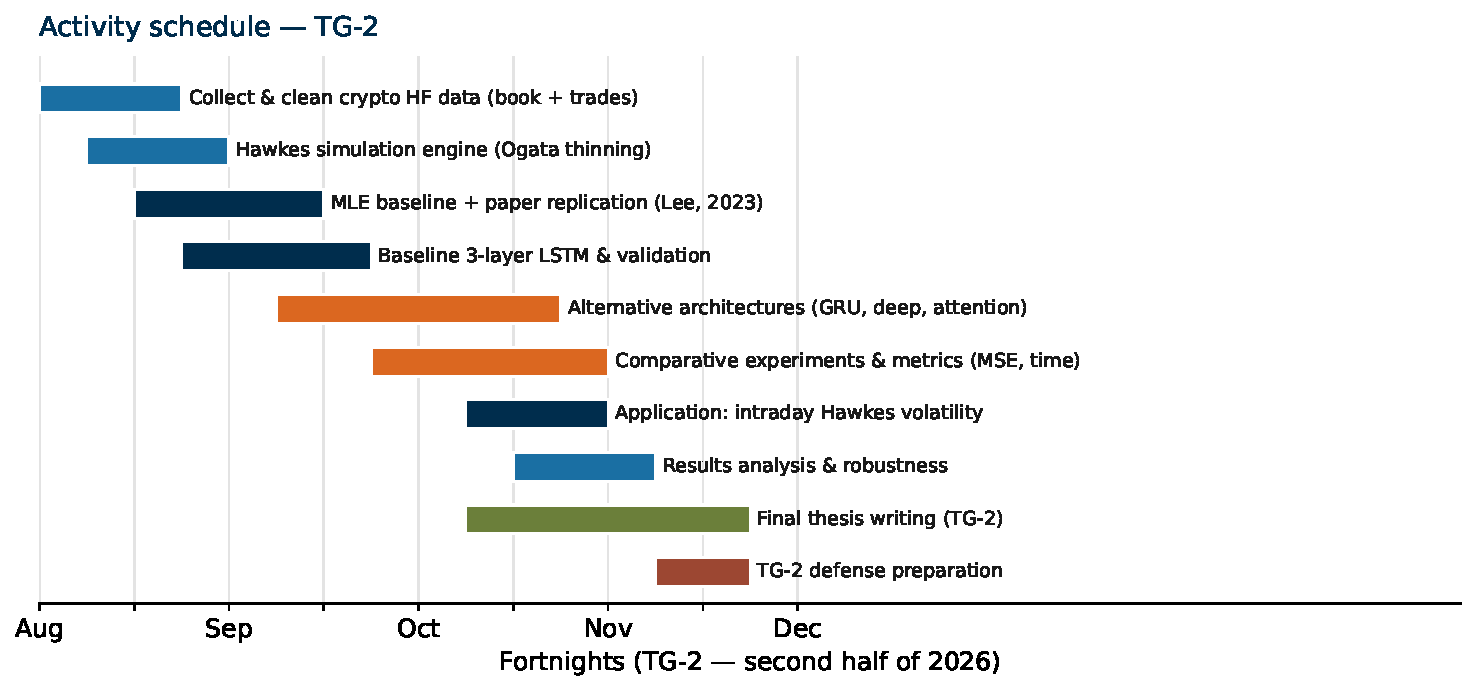
\includegraphics[width=0.88\linewidth]{figs/fig_gantt.pdf}
  \end{figure}
  \begin{center}
  {\footnotesize The core (data $\to$ simulator $\to$ MLE $\to$ LSTM) is delivered by mid-September.}
  \end{center}
\end{frame}

\begin{frame}{Next steps}
  \begin{block}{From the proposal (TG-1) to TG-2}
    \begin{itemize}
      \item Finish collecting and cleaning the high-frequency cryptocurrency data.
      \item Implement the Hawkes simulator and the MLE baseline.
      \item Reproduce Lee's (2023) LSTM and validate against the published results.
      \item Design and train the alternative architectures (GRU, deep, attention).
      \item Run the comparative experiments and the volatility application.
      \item Write the final thesis and prepare the TG-2 defense.
    \end{itemize}
  \end{block}
\end{frame}

% =====================================================================
\begin{frame}[allowframebreaks]{References}
  \footnotesize
  \begin{thebibliography}{99}
    \setbeamertemplate{bibliography item}[text]
    \bibitem{lee2023} LEE, K. \emph{Recurrent neural network based parameter estimation of Hawkes model on high-frequency financial data}. Finance Research Letters, v.\ 55, 103922, 2023.
    \bibitem{hawkes1971} HAWKES, A. G. \emph{Spectra of some self-exciting and mutually exciting point processes}. Biometrika, v.\ 58, n.\ 1, p.\ 83--90, 1971.
    \bibitem{leeseo2017} LEE, K.; SEO, B. K. \emph{Marked Hawkes process modeling of price dynamics and volatility estimation}. Journal of Empirical Finance, v.\ 40, p.\ 174--200, 2017.
    \bibitem{lee2024} LEE, K. \emph{Application of Hawkes volatility in the observation of filtered high-frequency price process in tick structures}. Applied Stochastic Models in Business and Industry, 2024.
    \bibitem{bouchaud2018} BOUCHAUD, J.-P.; BONART, J.; DONIER, J.; GOULD, M. \emph{Trades, Quotes and Prices: Financial Markets Under the Microscope}. Cambridge University Press, 2018.
    \bibitem{hardiman2013} HARDIMAN, S. J.; BERCOT, N.; BOUCHAUD, J.-P. \emph{Critical reflexivity in financial markets: a Hawkes process analysis}. The European Physical Journal B, v.\ 86, 442, 2013.
    \bibitem{bacry2013} BACRY, E.; DELATTRE, S.; MUZY, J.-F. \emph{Modelling microstructure noise with mutually exciting point processes}. Quantitative Finance, v.\ 13, p.\ 65--77, 2013.
    \bibitem{taddeo2024} TADDEO, M. M.; SALVI, L.; RIVERA-CASTRO, M. A. \emph{On the use of Hawkes processes to assess the jump frequency in cryptocurrency log-returns}. Brazilian Review of Finance, v.\ 22, n.\ 2, 2024.
    \bibitem{primo2018} PRIMO, G. O. \emph{Intraday clustering pattern of the Brazilian stock market: an exploratory analysis with Hawkes processes}. M.Sc.\ Dissertation --- UFPE, 2018.
    \bibitem{hochreiter1997} HOCHREITER, S.; SCHMIDHUBER, J. \emph{Long short-term memory}. Neural Computation, v.\ 9, p.\ 1735--1780, 1997.
    \bibitem{vaswani2017} VASWANI, A. et al. \emph{Attention is all you need}. Advances in Neural Information Processing Systems, v.\ 30, 2017.
    \bibitem{meieisner2017} MEI, H.; EISNER, J. M. \emph{The neural Hawkes process: a neurally self-modulating multivariate point process}. NeurIPS, v.\ 30, 2017.
    \bibitem{munitoke2011} MUNI TOKE, I. \emph{An introduction to Hawkes processes with applications to finance}. École Centrale Paris / BNP Paribas Chair, 2011.
    \bibitem{pacurar2006} PACURAR, M. \emph{Autoregressive conditional duration models in finance: a survey}. Dalhousie University, 2006.
    \bibitem{andersen2003} ANDERSEN, T. G.; BOLLERSLEV, T.; LABYS, P. \emph{Modeling and forecasting realized volatility}. Econometrica, v.\ 71, p.\ 579--625, 2003.
    \bibitem{kingma2014} KINGMA, D. P.; BA, J. \emph{Adam: a method for stochastic optimization}. arXiv:1412.6980, 2014.
    \bibitem{binance2024} BINANCE. \emph{Binance Public Data} — \texttt{data.binance.vision} (bookTicker, aggTrades). Accessed 2026.
  \end{thebibliography}
\end{frame}

% =====================================================================
\begin{frame}[plain]
  \centering
  \vspace{2cm}
  {\Huge \textbf{Thank you!}}\\[1cm]
  {\large Questions?}
\end{frame}

% =====================================================================
% BACKUP / APPENDIX SLIDES (not in the table of contents)
% =====================================================================
\appendix

\section{Appendix — Mathematical Background}

\begin{frame}{A.1 — Branching ratio, stationarity and memory}
  \begin{columns}[T]
    \begin{column}{0.52\textwidth}
      \begin{block}{Mean intensity}
        From $\phi(t)=\mu+\int_{-\infty}^t\Phi(t-u)\,\mathrm{d}N(u)$, take the stationary expectation ($\mathbb{E}[\mathrm{d}N]=\bar\phi\,\mathrm{d}u$):
        \[
          \bar\phi=\mu+\bar\phi\!\int_0^\infty\!\Phi(s)\,\mathrm{d}s=\mu+g\,\bar\phi,
        \]
        with $g:=\int_0^\infty\Phi(s)\,\mathrm{d}s$. Hence
        \[
          \boxed{\;\bar\phi=\frac{\mu}{1-g}\;}\quad(g<1).
        \]
      \end{block}
    \end{column}
    \begin{column}{0.48\textwidth}
      \begin{block}{Branching interpretation}
        \footnotesize
        Each event spawns offspring with intensity $\Phi$; the expected number of direct children is
        \[ \mathbb{E}[\#\text{children}]=\int_0^\infty\Phi(s)\,\mathrm{d}s=g. \]
        Mean family size (geometric series):
        \[ \bar S=1+g+g^2+\dots=\tfrac{1}{1-g}. \]
        Effective memory ($\Phi=\alpha e^{-\beta t}$): $\;\tau_{\text{eff}}\approx \tfrac{1}{\beta}\cdot\tfrac{1}{1-g}$ — diverges as $g\to1$.
      \end{block}
    \end{column}
  \end{columns}
\end{frame}

\begin{frame}{A.2 — From the scalar definition to the 2D marked intensity}
  \begin{block}{Three steps}
    \footnotesize
    \begin{enumerate}
      \item \textbf{Multivariate (2D):} types up (1)/down (2), each with $\lambda_i$; the kernel becomes a matrix
        $\;\lambda_i(t)=\mu_i+\sum_j\int_{-\infty}^t\Phi_{ij}(t-u)\,\mathrm{d}N_j(u).$
      \item \textbf{Symmetry + exponential:} $\Phi_{ij}(t)=\alpha_{ij}e^{-\beta t}$, $\;\boldsymbol\alpha=\big[\begin{smallmatrix}\alpha_1&\alpha_2\\ \alpha_2&\alpha_1\end{smallmatrix}\big]\Rightarrow \boldsymbol\Phi=\boldsymbol\alpha\circ\boldsymbol b(t)$.
      \item \textbf{Marks:} $\boldsymbol M(\mathrm{d}u\times\mathrm{d}z)$ records (time, jump $Z$); $\mathrm{d}N=\int_z\boldsymbol M$. The intensity ignores $z$; the \emph{price} uses $Z$ (hence ``marked'').
    \end{enumerate}
    Dropping the 2nd dimension and marks, with $\Phi=\alpha e^{-\beta t}$, recovers the Context definition.
  \end{block}
  \begin{alertblock}{Stationarity $\to$ what the network predicts}
    \footnotesize Spectral radius of $\int_0^\infty\boldsymbol\alpha\circ\boldsymbol b\,\mathrm{d}t=\boldsymbol\alpha/\beta<1$; eigenvalues $(\alpha_1\pm\alpha_2)/\beta$ give
    $\;(\alpha_1+\alpha_2)/\beta<1\;\Longleftrightarrow\;\beta-\alpha_1-\alpha_2>0$ — exactly the softplus target in Lee (2023).
  \end{alertblock}
\end{frame}

\begin{frame}{A.3 — The maximum-likelihood objective}
  \begin{block}{Bin argument}
    Over $[0,T]$ split into bins $\mathrm{d}t$: $P(\text{event})\approx\lambda\,\mathrm{d}t$, $P(\text{none})\approx e^{-\lambda\,\mathrm{d}t}$. The product over all bins gives
    \[
      L=\Big[\textstyle\prod_k\lambda(t_k)\Big]\,e^{-\int_0^T\lambda(u)\,\mathrm{d}u}
      \;\Rightarrow\;
      \log L=\sum_k\log\lambda(t_k)-\int_0^T\lambda(u)\,\mathrm{d}u.
    \]
  \end{block}
  \begin{block}{Multivariate marked form}
    \[
      L(T,\boldsymbol\theta)=\sum_{i=1}^{2}\Big[\sum_{t_{i,n}}\log\lambda_i(t_{i,n})-\int_0^T\!\lambda_i(u)\,\mathrm{d}u\Big],
    \]
    \footnotesize the first sum running over the type-$i$ event times. Substitute $\lambda_i(t)=\mu+\sum\alpha e^{-\beta(t-t_i)}$ and maximise over $\{\mu,\alpha_1,\alpha_2,\beta\}$ — an iterative, numerical step, replaced here by the network's learned inference.
  \end{block}
\end{frame}

\end{document}
